\documentclass[review,12pt,number]{elsarticle}
% Neurocomputing submission format: review = double spacing + line numbers;
% number = numeric citations with elsarticle-num. For a double-column
% production-style preview use [3p,times,number] or [5p,times,number].

\usepackage{amsmath,amssymb}
\usepackage{booktabs}
\usepackage{graphicx}
\usepackage{xcolor}
\usepackage{lineno}
\usepackage{url}
\graphicspath{{figs/}}

\newcommand{\todo}[1]{\textcolor{red}{[TODO: #1]}}
\newcommand{\delp}{DeLP}
\newcommand{\acc}{\mathrm{acc}}

\journal{Neurocomputing}

\begin{document}
\linenumbers

\begin{frontmatter}

\title{The Anchor Accumulation Problem:\\
Bounded Anchor Sets Recover Plasticity in
Usage-Localized Elastic Weight Consolidation}

\author[hnucm]{Ranxi Zhou}
\address[hnucm]{Hunan University of Chinese Medicine, 300 Xueshi Avenue,
Hanpu, Yuelu District, Changsha 410208, Hunan, China}
\cortext[cor1]{Corresponding author.}
\ead{zhouranxi@foxmail.com}

\begin{abstract}
Usage-localized elastic weight consolidation (\delp{}) protects dendritic
segments with per-neuron elastic anchors accumulated over the task sequence.
A decomposition of average retention,
$\bar a_T = \ell + \frac{T-1}{T}\,\mathrm{BWT}$, localized the cost of long
task sequences not in the architecture but in the \emph{learning term}
$\ell$: anchors accumulated under early tasks persist as an elastic drag on
later learning. We call this the \emph{anchor accumulation problem} and
study it directly by bounding the anchor stack at $M$ entries. Under four
eviction criteria we find that (i) a FIFO budget recovers $+4.5$ and
$+9.0$ points of final accuracy over unbounded \delp{} at $T{=}10$ and
$T{=}20$ tasks respectively ($n{=}10$ paired seeds, $t(9)>19$ in both
cases), recovering $+5.4$/$+15.2$ points of the learning term; (ii) the
budget is a distinct control knob from the elastic weight $\lambda$: both
trade protection for plasticity, but the budget controls the \emph{age
structure} of forgetting (which tasks are forgotten) while $\lambda$
controls its \emph{amount} (how much overall); (iii) eviction criteria
keyed to an anchor's current constraint mass fail catastrophically
--- they preserve stale anchors created before the budget first binds
(``grandfathering'') and evict anchors at birth, losing $-34.5$ BWT ---
whereas age-first criteria are immune; trace instrumentation of anchor
stacks shows the mechanism directly; and (iv) merging anchors removes exactly the redundant inter-anchor
cross terms --- the penalty drops one-sidedly by up to $64\%$ while
the accuracy trajectory remains indistinguishable from unbounded ---
separating the memory axis ($T \to M$ storage) from the plasticity
axis. A budget of $M{=}2$ raises final accuracy to
68.2\% at $T{=}10$, $+13.0$ points over unbounded \delp{}, and the effect
replicates on Fashion-MNIST at $n{=}10$ paired seeds ($+13.6$ points,
$t(9){=}18.3$) and on Split-CIFAR-100
with a ResNet-18 backbone, where at $T{=}20$ every bounded policy
outperforms unbounded stacking (up to $+5.0$ points, $t(9){=}7.1$) and
anchor-stack traces replicate the age-versus-mass mechanism
bit-for-bit. Single-anchor references bound the claim: plain EWC
maximizes the learning term at $3$--$5\times$ the forgetting, and
online EWC with a tuned discount ($\gamma{<}1$) overtakes the budget
at every grid cell --- revealing that discounting is itself a soft
bound, that soft and hard bounds fall on one curve relating
the learning term to the protected-mass horizon (log-linear at the
calibrated $\lambda$, monotone at every grid value), and
that bounding accumulated anchor mass, not the eviction mechanism, is
the active ingredient; on
Split-CIFAR-100 a no-protection baseline remains above every arm.
The explicit window's residual is an auditable, policy-selectable
protection set; bounded anchor sets turn a diagnosed failure mode
into a measured, tunable mechanism.
\end{abstract}

\begin{keyword}
continual learning \sep elastic weight consolidation \sep
catastrophic forgetting \sep dendritic computation \sep
stability--plasticity dilemma
\end{keyword}

\end{frontmatter}

% ============================================================
\section{Introduction}
% ============================================================
\label{sec:intro}

Elastic weight consolidation (EWC)~\cite{kirkpatrick2017} and its
variants protect important parameters by penalizing departure from
values that served previous tasks.
\delp{}~\cite{zhou2026delp} localizes this protection to dendritic
compartments and weights each neuron's penalty by its measured usage
under previous tasks; an audit of the method
established that usage weighting survives a parameter-budget cap
($+1.79$, $p{=}0.005$ at twenty tasks) while the full dendritic chain
adds almost nothing once baselines share the hidden activation.

The same audit exposed a structural cost: \delp{} appends one anchor
set (posterior means and Fisher estimates) per task, so the elastic
drag on optimization grows with the sequence length $T$.
A decomposition of average retention,
%
\begin{equation}
\label{eq:decomp}
\bar a_T \;=\; \ell \;+\; \frac{T-1}{T}\,\mathrm{BWT},
\end{equation}
%
separates the \emph{learning term} $\ell$ (how well each task is
acquired at its boundary) from the backward-transfer term.
At ten tasks the losses of unbounded \delp{} are concentrated in $\ell$:
anchors from early tasks persist as elastic drag long after the tasks
they protect have been consolidated, and this is a property of the
protection scheme, not of the architecture.


This paper treats the anchor stack itself as the object of study.
We bound it at $M$ entries and ask three questions:
\textbf{(Q1)} Can the learning term be recovered by bounding, and at
what stability cost?
\textbf{(Q2)} Is the budget a redundant knob (a non-linear re-scaling
of $\lambda$), or does it control something $\lambda$ cannot?
\textbf{(Q3)} If the stack must be bounded, \emph{which} anchors should
be evicted?

\paragraph{Contributions.}
\begin{enumerate}
\item \textbf{Bounded anchor sets.} We introduce a family of eviction
policies for anchor stacks and show that a FIFO budget recovers
$+4.5/+9.0$ points of final accuracy at $T{=}10/20$ over unbounded
\delp{} ($n{=}10$ paired seeds, $t(9){=}21.4/19.1$), by recovering
$+5.4/+15.2$ points of the learning term (Eq.~\ref{eq:decomp}).
A budget of $M{=}2$ reaches $68.2\%$ at $T{=}10$ ($+13.0$ over
unbounded), and the effect replicates on Fashion-MNIST ($+13.6$,
$n{=}10$ paired seeds) and
Split-CIFAR-100 (ResNet-18; at $T{=}20$ all six bounded policies beat
unbounded, up to $+5.0$ points, $t(9){=}7.1$).
\item \textbf{Two orthogonal knobs.} Through per-task accuracy
profiles we show the budget controls the \emph{age structure} of
forgetting (which tasks degrade) while $\lambda$ controls its total
amount; the profiles are qualitatively different shapes, not
re-scalings of one another (Fig.~\ref{fig:age}).
\item \textbf{A grandfathering failure mode.} Eviction criteria keyed
to an anchor's current constraint mass systematically evict anchors
\emph{at birth} (mass $\approx 0$ when the stack just changed) and
preserve stale pre-budget anchors; BWT collapses to $-34.5$.
Multiplicative age re-weighting does not fix this; an age-first,
mass-second criterion does. Trace instrumentation of anchor stacks
(Fig.~\ref{fig:stack}) shows the mechanism directly.
\item \textbf{A compressed memory axis.} Fisher-cosine merging
compresses the stack from $T$ to $M$ entries by removing exactly the
cross terms between merged anchors: penalty instrumentation shows a
one-sided drop (per-run maximum $18$--$64\%$) while the learned
trajectory stays indistinguishable from unbounded, separating memory
cost from plasticity.
\item \textbf{A mechanism-level boundary.} Sweeping online EWC's
discount $\gamma \in \{0.5, 0.9, 1\}$ shows a tuned discount overtakes
the budget on accuracy at matched forgetting, and that soft (discount)
and hard (window) bounds collapse onto one log-linear law between the
learning term and the protected-mass horizon: bounding accumulated
anchor mass is the active ingredient.
\end{enumerate}

% ============================================================
\section{Related work}
% ============================================================
\label{sec:related}

\begin{sloppypar}
\paragraph{Regularization-based continual learning.}
EWC~\cite{kirkpatrick2017} places a quadratic penalty around posterior
estimates of previous tasks; SI~\cite{zenke2017} accumulates
path-integral importances online; MAS~\cite{aljundi2018} estimates
sensitivity unsupervised. Anchor accumulation is not specific to
\delp{}: any scheme that stores per-task quadratics pays storage
$O(T)$ and, if all terms persist at full weight, an increasingly
rigid objective. Online EWC~\cite{chaudhry2018} addresses the storage
axis by collapsing the stack into a single running posterior; with a
discount $\gamma{<}1$ its Fisher mass is geometrically bounded, which
makes it a \emph{soft} bound on the same accumulated mass we diagnose
(Sec.~\ref{sec:exp-references}). Bounded anchor sets are complementary:
they keep per-task terms and bound their number.
\end{sloppypar}
\paragraph{Parameter isolation and budgeting.}
PackNet~\cite{mallya2018} and HAT~\cite{serra2018} budget capacity
explicitly. Our contribution differs: the budgeted object is the
\emph{protection} state, not the network capacity, and eviction can
be nearly free when the penalty is combined correctly (merge).

\paragraph{Dendritic computation.}
Active-dendrite networks~\cite{iyer2022,onasch2026} provide the
architectural substrate; \delp{}'s audit~\cite{zhou2026delp}
established which part of the dendritic chain carries the benefit.

% ============================================================
\section{Background: \delp{} and anchor accumulation}
% ============================================================
\label{sec:background}

\paragraph{Setup.}
A network is trained on a sequence of $T$ tasks (permuted MNIST /
Fashion-MNIST). \delp{} freezes dendritic segments unused by the
current task and adds, after each task $t$, an anchor set
$\mathcal{A}_t = \{(\theta_t, F_t)\}$ (parameter snapshot and Fisher
diagonal). The protection objective during task $t$ is
%
\begin{equation}
\label{eq:delp}
\mathcal{L}_t(\theta) \;=\; \mathcal{L}_t^{\text{task}}(\theta)
\;+\; \frac{\lambda}{2}\sum_{k<t}\sum_i F^{(k)}_i
      \,(\theta_i - \theta^{(k)}_i)^2 ,
\end{equation}
%
where the inner sum runs over the accumulated stack
$\mathcal{A}_1, \dots, \mathcal{A}_{t-1}$: the penalty is
\emph{unbounded} in $T$, both in storage and in constraint mass.

\paragraph{Where the cost lands.}
Following~\cite{zhou2026delp}, average retention decomposes as
Eq.~\ref{eq:decomp}. % cite numbers: at T=10 unbounded DeLP:
% acc 55.3, BWT -5.5, ell 60.2; at T=20: 33.7 / -4.4 / 37.9
At $T{=}10$ the learning term of unbounded \delp{} sits $5.4$ points
below its $T{=}5$ value, and the gap widens with $T$;
anchored identity Eq.~\ref{eq:decomp} attributes the gap to $\ell$,
not BWT. We call this the \emph{anchor accumulation problem}.

% ============================================================
\section{Bounded anchor sets}
% ============================================================
\label{sec:method}

\paragraph{Budgeted stacks.}
We replace the unbounded stack with a bounded one of size $M$.
After appending the anchor for task $t$, if $|\mathcal{A}| > M$ an
\emph{eviction policy} removes or combines entries:
%
\begin{equation}
\label{eq:budget}
\mathcal{A} \leftarrow \mathsf{evict}_\pi\!\left(
\mathcal{A} \cup \{(\theta_t, F_t)\},\, M \right).
\end{equation}

\paragraph{Policies.}
Table~\ref{tab:policies} defines the six policies we compare. They
span the design space along one axis: \emph{what signal drives the
choice} --- age (fifo), chance (random), current constraint mass
(redun), pairwise redundancy (merge), or combinations of age and
mass (agew, agew2).

\begin{table}[t]
\centering\small
\caption{Eviction policies for a stack over budget. Constraint mass
$m_k = \sum_i F^{(k)}_i (\theta^{\text{now}}_i-\theta^{(k)}_i)^2$ is
measured at eviction time.}
\label{tab:policies}
\begin{tabular}{llp{8.2cm}}
\toprule
Policy & Key & Rule (when $|\mathcal{A}|>M$) \\
\midrule
unbounded & --- & never evict (original \delp{}) \\
fifo      & age & evict the oldest anchor \\
random    & --- & evict uniformly at random \\
redun     & mass & evict $\arg\min_k m_k$ \\
agew      & mass $\times$ age & evict $\arg\min_k m_k \cdot (k{+}1)$,
    oldest $k{=}0$ \\
agew2     & age $\to$ mass & evict oldest anchor with below-median $m_k$;
    fallback fifo \\
merge     & redundancy & merge the pair with most similar $F$
    (cosine): $F \leftarrow F_i + F_j$, $\theta \leftarrow$ weighted
    mean; repeat \\
\bottomrule
\end{tabular}
\end{table}

\begin{sloppypar}
\paragraph{Instrumentation.}
Each anchor carries an \emph{origin} tag (the task that created it),
and we record the surviving-origin set after every phase
(\texttt{survivor\_history}). This turns the eviction dynamics into a
directly observable object (Fig.~\ref{fig:stack}).
\end{sloppypar}

% ============================================================
\section{Experiments}
% ============================================================
\label{sec:exp}

\paragraph{Protocol.}
Permuted-MNIST and Fashion-MNIST, $T \in \{10, 20\}$; architecture,
optimizer, permutation generation, and evaluation identical to the
\delp{} audit protocol~\cite{zhou2026delp}; $\lambda{=}5000$ unless stated. Every arm runs at the pipeline's
\emph{default} hidden-layer gain --- the uncalibrated condition of the
audit's calibration protocol~\cite{zhou2026delp} --- and no arm is
gain-tuned within this study; since the gain is shared, the confound
the audit documented (a single gain scalar moves accuracy by more than
the entire method) cannot differentially favor any arm, only shift all
arms together. Paired comparisons use identical seeds.
Budgets $M \in \{2, 5\}$ anchor the main grid; a seven-point
dose--response sweep $M \in \{2,3,4,5,6,8,10\}$ ($T{=}20$,
$\lambda{=}5000$; Sec.~\ref{sec:exp-knobs}) fills the interior, and no
$M$ was tuned post hoc.
Section~\ref{sec:exp-cifar} states the Split-CIFAR-100 protocol
separately (different backbone and protection pathway).

\subsection{Bounding recovers plasticity (Q1)}
\label{sec:exp-main}

\begin{table}[t]
\centering\small
\caption{Paired fifo--unbounded deltas, $M{=}5$, $\lambda{=}5000$,
$n{=}10$ seeds.}
\label{tab:paired}
\begin{tabular}{lccc}
\toprule
Arm & $\Delta\acc$ & $t(9)$ & $\Delta$BWT \\
\midrule
fifo $T{=}10$ & $+4.51\pm0.67$ & $21.4$ & $-1.50\pm0.49$ \\
fifo $T{=}20$ & $+8.98\pm1.49$ & $19.1$ & $-7.20\pm1.97$ \\
\bottomrule
\end{tabular}
\end{table}

\begin{table}[t]
\centering\small
\caption{Policy grid, $M{=}5$, $\lambda{=}5000$, mean $\pm$ sd over
$n{=}3$ seeds. $\ell$ = learning term (mean accuracy at task
boundaries). agew is bit-identical to redun, as predicted in
Sec.~\ref{sec:exp-criteria}.}
\label{tab:grid}
\begin{tabular}{llccc}
\toprule
$T$ & Arm & BWT & $\acc$ & $\ell$ \\
\midrule
10 & unbounded & $-5.5\pm0.6$   & $55.3$ & $60.2$ \\
10 & fifo      & $-6.6\pm0.9$   & $59.7$ & $65.6$ \\
10 & random    & $-9.1\pm2.6$   & $60.2$ & $68.4$ \\
10 & redun     & $-18.3\pm0.8$  & $53.6$ & $70.1$ \\
10 & agew      & $-18.3\pm0.8$  & $53.6$ & $70.1$ \\
10 & agew2     & $-8.4\pm0.9$   & $60.8$ & $68.3$ \\
10 & merge     & $-5.5\pm0.6$   & $55.3$ & $60.3$ \\
\midrule
20 & unbounded & $-4.4\pm1.0$   & $33.7$ & $37.9$ \\
20 & fifo      & $-10.2\pm1.9$  & $43.4$ & $53.1$ \\
20 & random    & $-13.5\pm0.4$  & $42.0$ & $54.8$ \\
20 & redun     & $-30.2\pm0.4$  & $36.3$ & $65.0$ \\
20 & agew      & $-30.2\pm0.4$  & $36.3$ & $65.0$ \\
20 & agew2     & $-16.5\pm0.3$  & $42.3$ & $58.0$ \\
20 & merge     & $-4.5\pm0.9$   & $33.6$ & $37.9$ \\
\bottomrule
\end{tabular}
\end{table}

Table~\ref{tab:paired}: a FIFO budget at $M{=}5$ trades $1.5/7.2$ points
of BWT for $+4.5/+9.0$ accuracy. The mechanism is the learning term:
$\ell$ rises by $+5.4$ and $+15.2$, exactly the recovery predicted if
accumulated elastic drag were the binding constraint
(Sec.~\ref{sec:background}); the grid in Table~\ref{tab:grid} shows the
same signature for every bounded arm.
Eq.~\ref{eq:decomp} is an accounting identity, so the decomposition
alone is not evidence; the causal claim rests on the eviction traces
(Sec.~\ref{sec:exp-criteria}) and on the $\lambda$-by-budget
interaction (Sec.~\ref{sec:exp-knobs}), which localize \emph{when}
the learning term moves --- namely when anchors are actually retired.
Corrected SI at $T{=}10$ ($\lambda{=}100$) reaches $40.3\%$.

\paragraph{Single-anchor references.}
\label{sec:exp-references}
Because the diagnosis targets the \emph{stack}, we also ran two
protection schemes that cannot accumulate one, on the identical
architecture, protocol, and $\lambda$ grid ($n{=}10$ paired seeds):
plain EWC, which keeps only the most recent task's Fisher and anchor
(no accumulation, no running Fisher update --- distinct from the
original accumulated variant of~\cite{kirkpatrick2017}), and online
EWC \cite{chaudhry2018} with $\gamma \in \{0.5, 0.9, 1\}$, which
collapses the stack into a single running posterior with geometrically
discounted Fisher accumulation. All arms share the identical
$\lambda$ grid and are compared at each scheme's best grid value, so
no scheme is disadvantaged by another's tuning. Plain EWC posts the
highest final accuracy
of any arm ($68.3$--$71.1$ at $T{=}10$, $56.4$--$59.4$ at $T{=}20$,
best at $\lambda{=}1000$) by maximizing $\ell$ ($81$--$85$): with no
stack there is no accumulation --- and no retention either, at
$3$--$5\times$ the forgetting of unbounded \delp{} (BWT
$-15.8/-25.7$ at its best $\lambda$ vs.\ $-5.5/-4.4$). Under the
final-accuracy metric the learning-term dominance outweighs retention;
a reader who weights BWT equally would rank it last. Online EWC at its
best grid value ($\lambda{=}1000$) reaches $67.5/46.0$: at $T{=}10$ it
is statistically indistinguishable from \delp{}-fifo at the same
$\lambda$ ($67.4$; paired $t(9){=}-0.3$); at $T{=}20$ fifo is $+3.5$
ahead ($t(9){=}7.0$). A collapsed posterior thus recovers most of the
plasticity, but it posts neither the best long-sequence accuracy nor,
by construction, any anchor accumulation problem to cure. Its
forgetting is not unstructured: per-task forgetting (peak minus
final accuracy; $T{=}20$, $\lambda{=}1000$, $n{=}10$) concentrates on
older tasks for every arm, with drop--age correlations of $-0.94$
(plain), $-0.79$ (\delp{}-fifo), $-0.70$ (online EWC), and $-0.43$
(unbounded). Sweeping the discount shows that the collapsed posterior
does have an age knob after all: lowering $\gamma$ to $0.9$ and $0.5$
raises $\ell$ from $51.1$ to $56.6$ and $76.1$ ($T{=}20$,
$\lambda{=}1000$), and at $\gamma{=}0.5$ online EWC overtakes
\delp{}-fifo at every grid cell we tested (paired $+4.7$ to $+7.9$,
all $|t(9)|\geq10.4$) at essentially matched BWT ($-19.5$ vs.\
$-19.7$). Discounting, however, is itself a bound: with geometrically
decayed Fishers the accumulated mass converges to an effective horizon
of ${\approx}\,1/(1-\gamma)$ tasks, so $\gamma{<}1$ is a \emph{soft}
counterpart of the eviction window, and the two mechanisms turn out to
be interchangeable points on one curve. Across all five bounded-mass
arms at $\lambda{=}1000$, $\ell$ is log-linear in the protected
horizon $h$ ($h{=}1$ plain, $h{=}2$ for $\gamma{=}0.5$, $h{=}5$ for
the window, $h{=}10$ for $\gamma{=}0.9$, $h{=}20$ unbounded):
$\ell \approx 84 - 11\ln h$ with $R^2{=}0.99$ --- a fit that holds for
every seed individually (per-seed $R^2 \geq 0.98$, slope
$-10.9\pm0.6$), replicates at $T{=}10$ ($R^2{=}1.00$), and whose
ordering is monotone at every grid $\lambda$ (mean-fit $R^2$
$0.99/0.94/0.80$ as $\lambda$ tightens). Bounding accumulated anchor
mass --- not
the mechanism that enforces the bound --- is the active ingredient,
and the soft bound is the stronger remedy on final accuracy in this
regime. What the explicit window retains is auditability and
policy-level choice: its protection set is discrete and named by the
survivor trace; the forgetting profile it produces is the one the
trace predicts ($8.6$ on recent tasks vs.\ $27.7$ on the evicted
oldest); and the eviction key can be swapped (age, mass) or the stack
merged without touching the update rule. The object studied here
remains the stack; the budget is one of two cures, and on this
benchmark the simpler one wins.

\subsection{Budget vs.\ $\lambda$: two orthogonal knobs (Q2)}
\label{sec:exp-knobs}

Fig.~\ref{fig:pareto} shows the Pareto plane; Fig.~\ref{fig:age} the
per-task accuracy profiles; Table~\ref{tab:lambda} the $\lambda$
interaction.

\paragraph{Dose--response.}
A seven-point sweep at $T{=}20$, $\lambda{=}5000$ ($n{=}10$) shows the
budget's effect is monotone across the whole interior, not an artifact
of two extreme points: final accuracy $52.6, 49.0, 44.7, 42.0, 40.1,
36.3, 35.1$ for $M{=}2,3,4,5,6,8,10$, with BWT recovering
$-24.3 \to -5.2$ as the window widens toward $M{=}10$; every $M$
remains significantly above unbounded ($38.6$; paired $t(9)$ from
$27.2$ at $M{=}2$ down to $8.0$ at $M{=}10$, approaching the window's
own limit).

\begin{figure}[t]
\centering
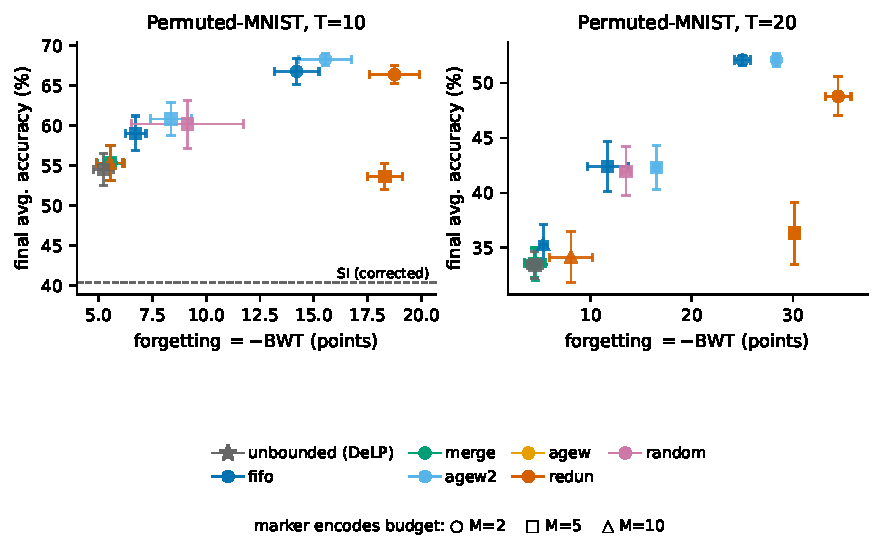
\includegraphics[width=\linewidth]{fig1_pareto.pdf}
\caption{Accuracy--forgetting trade-off on Permuted-MNIST. Color
encodes policy; marker encodes budget $M$. Error bars: sd over seeds
($n{=}10$ for unbounded/fifo $M{=}5$; else $n{=}3$). The smaller
budget $M{=}2$ trades BWT for accuracy at both budgets in the same
direction; merge coincides with
unbounded at every $M$; redun sits dominated.}
\label{fig:pareto}
\end{figure}

\begin{table}[t]
\centering\small
\caption{$\lambda$ interaction ($M{=}5$, $n{=}10$ paired seeds): the
fifo advantage is positive at every $\lambda$ and grows with $T$
(all paired $t(9)\geq 11$, $p<10^{-6}$).}
\label{tab:lambda}
\begin{tabular}{llcccc}
\toprule
$\lambda$ & $T$ & unbounded BWT/$\acc$ & fifo BWT/$\acc$ & $\Delta\acc$ \\
\midrule
1000  & 10 & $-11.6 / 63.9$ & $-10.8 / 67.4$ & $+3.5$ \\
5000  & 10 & $-5.2 / 54.5$  & $-6.7 / 59.0$  & $+4.5$ \\
20000 & 10 & $-1.9 / 49.0$  & $-4.0 / 53.1$  & $+4.1$ \\
1000  & 20 & $-13.8 / 38.6$ & $-19.7 / 49.5$ & $+10.9$ \\
5000  & 20 & $-4.5 / 33.4$  & $-11.7 / 42.4$ & $+9.0$ \\
20000 & 20 & $-1.5 / 29.8$  & $-6.6 / 37.3$  & $+7.5$ \\
\bottomrule
\end{tabular}
\end{table}

The fifo advantage is robust to the choice of $\lambda$: even granting
unbounded \delp{} its best grid value at each $T$ ($\lambda{=}1000$, the
value at which unbounded is strongest at $T{=}20$), fifo retains a
$+10.9$-point advantage there (and $+3.5$ at $T{=}10$). That the
unbounded-optimal $\lambda$ must drift downward as $T$ grows is itself
a symptom of accumulating rigidity: the protection budget has to be
relaxed sequence-wide to compensate for anchors that a bounded scheme
would simply retire.

Both knobs move the system along a protection--plasticity spectrum,
but they are not re-parameterizations of one another. At matched
plasticity recovery, the two knobs produce \emph{different age
structures} of forgetting (Fig.~\ref{fig:age}):
$\lambda{=}1000$ scales down protection uniformly --- the profile
keeps its steep age gradient ($38.5$-point spread, oldest tasks at
65--83\%, newest at 45--51\%) --- while fifo $M{=}2$
redistributes forgetting onto the oldest tasks, flattening the
profile ($25.7$-point spread).
No value of $\lambda$ produces the flat profile, and no value of $M$
produces the uniform scaling.

\begin{figure}[t]
\centering
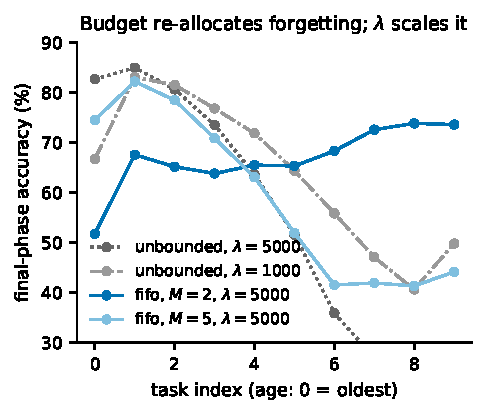
\includegraphics[width=0.62\linewidth]{fig2_ageprofile.pdf}
\caption{Final-phase accuracy per task ($T{=}10$, $n{=}10$).
$\lambda$ knobs (gray) translate the profile; budget knobs (blue)
flatten it: forgetting is re-allocated to the oldest tasks.}
\label{fig:age}
\end{figure}

\subsection{Which anchors to evict (Q3)}
\label{sec:exp-criteria}

\begin{figure*}[t]
\centering
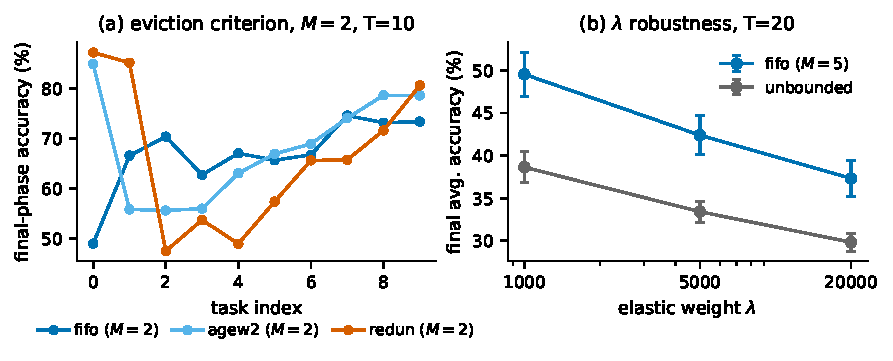
\includegraphics[width=\linewidth]{fig3_criteria.pdf}
\caption{(a) Mass-keyed eviction (redun) grandfather-protects the
first $M$ tasks and erases the middle; age-first criteria (fifo,
agew2) spread the cost. (b) The fifo advantage over unbounded holds
at every $\lambda$.}
\label{fig:criteria}
\end{figure*}

\paragraph{The grandfathering trap.}
Mass-keyed eviction is not a straw man: ``drop the anchor that
constrains least'' is the natural heuristic, homologous to
low-sensitivity-first intuitions in pruning and in MAS-style
importance estimates, and it is what a practitioner would try first.
Its systematic failure is the point. Constraint mass $m_k$
(Table~\ref{tab:policies}) is measured at
eviction time and is a function of staleness: anchors created before
the budget first binds have $\theta^{(k)}$ far from
$\theta^{\text{now}}$ and permanently large $m_k$; anchors created
\emph{after} the stack is full have $\theta^{(k)} \approx
\theta^{\text{now}}$ and $m_k \approx 0$. Mass-keyed eviction
therefore preserves exactly the stalest anchors and evicts new ones
\emph{at birth}: redun's stack freezes at
$\{\mathcal{A}_1, \mathcal{A}_2\}$ (Fig.~\ref{fig:stack}), the first
two tasks keep strong protection (87/85\% final accuracy at
$M{=}2$), and tasks created later lose all protection within one
phase (final accuracy 19--25\%), driving BWT to $-34.5$ at $T{=}20$
despite the \emph{highest} $\ell$ of any arm.

\paragraph{Re-weighting mass by age does not help.}
agew (mass $\times$ age-rank) is \emph{bit-identical} to redun across
all seeds and configurations: mass differences span orders of
magnitude and swamp the age factor, so the argmin never flips.
Any criterion with mass as the primary key inherits the trap.

\paragraph{Age-first criteria close the matrix.}
agew2 (oldest anchor with below-median mass; fallback fifo) behaves
like fifo ($\pm 1.5$ points): at $M{=}2$ its stack is
$\{\mathcal{A}_1, \mathcal{A}_T\}$ --- the oldest anchor's mass is
always above median and survives, everything in between dies at
birth. Table~\ref{tab:criteria} summarizes the resulting
$2{\times}2$: the primary key, not the secondary signal, determines
whether a criterion works.

\begin{table}[t]
\centering\small
\caption{Criteria $2{\times}2$: primary key (rows) $\times$ secondary
signal (columns). Only age-first criteria avoid the trap.
$T{=}10$/$T{=}20$ BWT and accuracy, $M{=}2$ or $M{=}5$ as marked,
$n{=}3$.}
\label{tab:criteria}
\begin{tabular}{lll}
\toprule
Primary key & Secondary & Outcome \\
\midrule
mass  & ---   & redun: grandfathering, BWT $-30.2$ ($M5$, T20) \\
mass  & $\times$ age & agew $\equiv$ redun (bit-identical) \\
age   & ---   & fifo: sliding window, BWT $-10.2$ ($M5$, T20) \\
age   & median mass & agew2 $\approx$ fifo ($\pm1.5$ pts) \\
\bottomrule
\end{tabular}
\end{table}

\begin{figure*}[t]
\centering
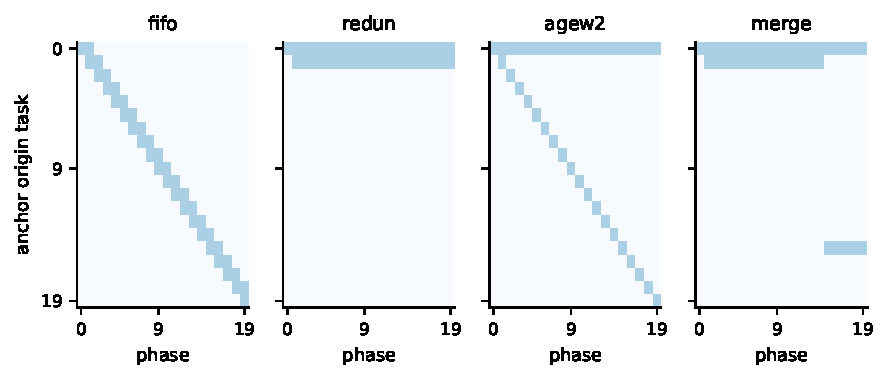
\includegraphics[width=\linewidth]{fig4_stacktrace.pdf}
\caption{Anchor-stack composition over the task sequence ($T{=}20$,
$M{=}2$, seed 0; identical for other seeds). Each column lists which
anchors (by creation task) are alive at the end of each phase. fifo
is a pure sliding window; redun freezes on the first two anchors
(evicting every later anchor at birth); agew2 protects the oldest and
the newest; merge partially grandfather-protects.}
\label{fig:stack}
\end{figure*}

\subsection{Memory without behavior change: merge}
\label{sec:exp-merge}

Merging the most Fisher-similar pair removes exactly the cross term
between the merged anchors. Penalty instrumentation over $40$ runs
($T \in \{10,20\}$, $M \in \{2,5\}$, $n{=}10$; exactly $T{-}M$ merges
per run) makes the change quantitative: the penalty decreases
one-sidedly --- never increases --- with per-run maximum relative
drops of $43$--$45\%$ at $M{=}2$ (worst case $64\%$) and $18$--$34\%$
at $M{=}5$, and $77\%$ of individual merges move the penalty at all.
The removed mass is precisely the redundancy the merge detected; the
accuracy trajectory nonetheless remains indistinguishable from
unbounded at every $M$ (Table~\ref{tab:grid}) while storing
$M \ll T$ anchors ($-75\%$ at $T{=}20$, $M{=}5$).
Merge and fifo are complementary: merge buys storage at a measured,
behaviorally invisible penalty reduction but recovers no plasticity;
fifo buys plasticity at a BWT price but no storage reduction.

\subsection{Generality check: Fashion-MNIST}
\label{sec:exp-fashion}

Fashion-MNIST, $T{=}10$, $n{=}10$ paired seeds: unbounded
$35.1\pm1.3$; fifo $M{=}5$ $38.1\pm1.7$ ($+2.9$, $t(9){=}11.5$); fifo
$M{=}2$ $48.7\pm2.5$ ($+13.6$, $t(9){=}18.3$). The budget
effect replicates and amplifies as the budget shrinks.

\subsection{Generalization to Split-CIFAR-100}
\label{sec:exp-cifar}

\paragraph{Protocol.}
Split-CIFAR-100, $T \in \{10, 20\}$ (10 classes per task), ResNet-18
adapted to $32{\times}32$ inputs with GroupNorm in place of BatchNorm
--- running statistics are buffers that drift under later tasks and
silently destroy protected tasks while the anchored weights themselves
are held fixed, so they are excluded by design. Evaluation and training
are task-incremental with a masked softmax head: each task computes its
loss only over its own 10 classes, so head rows of past tasks receive
no gradient and are protected by construction; anchors therefore cover
the backbone only, and forgetting can propagate exclusively through
the shared trunk --- exactly the pathway the anchor stack governs.
Fisher diagonals are rescaled to unit global mean (one scalar over all
parameters), making $\lambda$ backbone-independent; gradients are
clipped at norm 5. SGD, five epochs per task, $\lambda{=}0.1$ (chosen
by an independent calibration sweep on unbounded \delp{} only),
$n{=}10$ seeds; eviction policies, origin instrumentation, and paired
evaluation identical to the MNIST experiments. Unbounded \delp{} never
evicts, so its $M$ is inert (final stack size $T$ in every run); it is
materialized once per $T$ and serves as the reference for both
budgets. All CIFAR comparisons are task-incremental (masked head);
absolute accuracies are therefore not comparable to the
class-incremental Split-CIFAR-100 literature, and every claim in this
section is a within-family, same-protocol paired comparison.

\begin{table}[t]
\centering\small
\caption{Split-CIFAR-100, $\lambda{=}0.1$: final accuracy, mean
$\pm$ sd over $n{=}10$ seeds; parenthesized values are the paired
difference $\Delta\acc$ against unbounded \delp{} at the same seed
(quoted in text with paired $t(9)$ where significant).}
\label{tab:cifar}
\setlength{\tabcolsep}{4pt}
\footnotesize
\begin{tabular}{lcccc}
\toprule
& \multicolumn{2}{c}{$T{=}10$} & \multicolumn{2}{c}{$T{=}20$} \\
\cmidrule(r){2-3}\cmidrule(l){4-5}
Policy & $M{=}2$ & $M{=}5$ & $M{=}2$ & $M{=}5$ \\
\midrule
unbounded & \multicolumn{2}{c}{$23.3\pm2.6$} & \multicolumn{2}{c}{$29.8\pm4.2$} \\
fifo   & $24.8\pm2.8$ ($+1.5$) & $23.5\pm2.6$ ($+0.2$) &
         $\mathbf{34.8\pm4.8}$ ($+5.0$) & $32.2\pm4.3$ ($+2.4$) \\
random & $24.7\pm2.4$ ($+1.5$) & $22.4\pm2.7$ ($-0.9$) &
         $33.4\pm3.9$ ($+3.6$) & $32.2\pm4.7$ ($+2.4$) \\
redun  & $24.0\pm2.5$ ($+0.7$) & $23.6\pm2.0$ ($+0.3$) &
         $33.2\pm4.7$ ($+3.4$) & $32.9\pm3.3$ ($+3.1$) \\
merge  & $22.3\pm1.7$ ($-1.0$) & $21.8\pm3.2$ ($-1.5$) &
         $30.8\pm5.2$ ($+1.0$) & $29.3\pm3.4$ ($-0.5$) \\
agew   & $24.0\pm3.8$ ($+0.7$) & $22.7\pm3.4$ ($-0.6$) &
         $34.0\pm4.3$ ($+4.2$) & $31.6\pm3.7$ ($+1.8$) \\
agew2  & $23.7\pm2.6$ ($+0.4$) & $22.3\pm3.3$ ($-1.0$) &
         $32.5\pm3.7$ ($+2.7$) & $31.1\pm3.4$ ($+1.3$) \\
\bottomrule
\end{tabular}
\end{table}

\begin{sloppypar}
\paragraph{The budget effect strengthens with $T$ on natural images.}
At $T{=}20$ every bounded policy outperforms unbounded stacking
(Table~\ref{tab:cifar}): fifo $+5.0$ ($t(9){=}7.1$), agew $+4.2$
($t{=}7.3$), random $+3.6$ ($t{=}9.2$), redun $+3.4$ ($t{=}4.0$);
at $T{=}10$ the effect is marginal, about $+1.5$ points at
$t(9)\approx 2$.
The dose--response matches the mechanism: anchor drag accumulates
with sequence length, so the benefit of bounding it should grow with
$T$. As in Sec.~\ref{sec:exp-main}, the gain lands in the learning
term: fifo $M{=}2$ raises $\ell$ from $31.4$ to $36.8$ while BWT
moves only from $-1.7$ to $-2.1$ --- the budget buys plasticity, the
trade Eq.~\ref{eq:decomp} predicts. The decomposition itself is exact
on these runs: over all 260 CIFAR records,
$|\bar a_T - (\ell + \frac{T-1}{T}\mathrm{BWT})|$ never exceeds
$5\times10^{-3}$, i.e.\ the rounding of two-decimal reporting.
\end{sloppypar}

\paragraph{A no-protection reference.}
$\lambda{=}0$ (plain SGD, same protocol, $n{=}10$ paired seeds)
reorders the picture and must be reported: $27.0\pm1.7$ at $T{=}10$
and $36.9\pm3.4$ at $T{=}20$ --- above every \delp{} arm, including
fifo $M{=}2$ ($+2.1$, $t(9){=}1.5$, not significant). The
decomposition explains why: protection roughly halves the learning
term ($\ell$ is $25.7$ and $31.4$ at $T{=}10/20$ for unbounded \delp{},
vs.\ $46.1$ and $64.3$ at $\lambda{=}0$), while in this regime
retention is nearly free to
forgo --- even the large BWT of the unprotected arm ($-21.3/-28.9$)
costs less than the $\ell$ it gains. Under task-incremental evaluation
with a fixed masked head, trunk features are shared across tasks and
trunk drift is cheap; regularization-based protection at any $\lambda$
is then a net tax on accuracy. The budget effect remains real within
the protected family, but on this benchmark bounding is necessary, not
sufficient: protection itself must be checked against a no-protection
reference before the mechanism is credited.

\paragraph{Stack traces replicate bit-for-bit.}
At $T{=}20$, $M{=}2$, all ten seeds agree: fifo's stack is the sliding
window $\{\mathcal{A}_{T-1}, \mathcal{A}_{T}\}$; redun freezes on
$\{\mathcal{A}_1, \mathcal{A}_2\}$ (grandfathering); agew inherits the
same freeze (eviction-time mass swamps the age factor); agew2 holds
$\{\mathcal{A}_1, \mathcal{A}_{T}\}$ in 6/10 seeds (the age-primary
hybrid); merge grandfather-protects partially. The mechanism isolated
on Permuted-MNIST (Fig.~\ref{fig:stack}) is not an artifact of that
domain (Fig.~\ref{fig:stackcifar}).

\begin{figure*}[t]
\centering
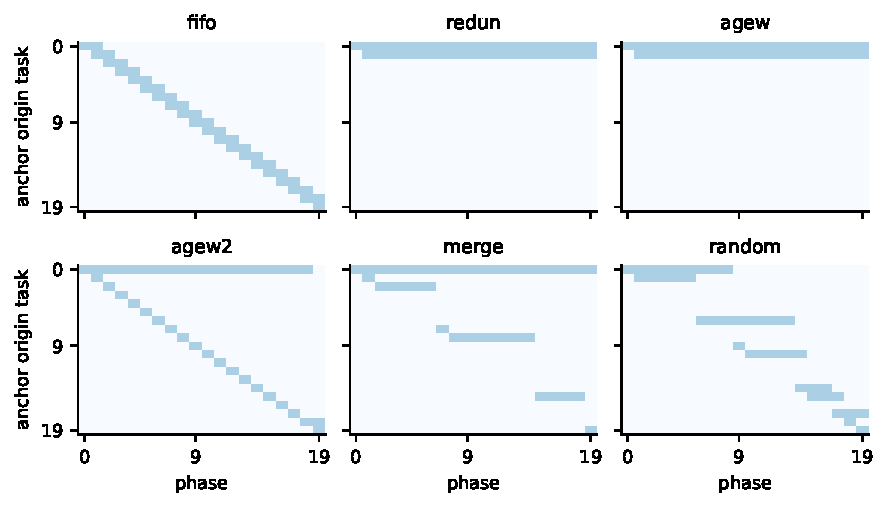
\includegraphics[width=\linewidth]{fig5_cifar_stacktrace.pdf}
\caption{Anchor-stack composition on Split-CIFAR-100 ($T{=}20$,
$M{=}2$, seed 0; all seeds agree on the final sets). Same rendering as
Fig.~\ref{fig:stack}. fifo is a sliding window; redun and agew freeze
on the first anchors (grandfathering); agew2 pairs the oldest with the
newest; merge partially grandfather-protects; random walks down.}
\label{fig:stackcifar}
\end{figure*}

\paragraph{A boundary condition on the mass-keyed failure.}
Unlike on MNIST, the \emph{secondary} effect --- \emph{which}
criterion evicts --- is weak here: fifo $-$ redun is $+1.6$
($t(9){=}2.0$) at $T{=}20$, $M{=}2$, and agew2 $-$ redun is slightly
negative. The reason is structural: under masked-CE training,
forgetting propagates only through the shared trunk, whose low layers
are described similarly by every task's Fisher diagonal; even the
stale anchors $\{\mathcal{A}_1, \mathcal{A}_2\}$ constrain features
later tasks still use, so grandfathering them costs little.
Mass-keyed eviction fails when anchors describe task-specific
structure that goes stale; the primary effect of bounding (recovering
plasticity) survives, while the relative cost of grandfathering
scales with how much low-level structure tasks share --- a testable
prediction for domain-incremental sequences, where the gap should
re-open.

% ============================================================
\section{Discussion}
% ============================================================
\label{sec:discussion}

\paragraph{Why bounding works.}
Eq.~\ref{eq:decomp} says total retention is learning plus transfer;
unbounded stacks tax learning with stale constraints. A FIFO window
keeps only the freshest $M$ constraints, whose $\theta^{(k)}$ are
near $\theta^{\text{now}}$ and whose Fisher mass is relevant to the
current basin: the penalty constrains what actually needs
constraining.

\paragraph{The mass signal is not useless --- it is mis-keyed.}
redun asks ``which anchor constrains least \emph{now}?''; the honest
answer at eviction time is ``the one just created'', which is exactly
the wrong anchor to drop. agew2 shows mass adds marginal, unstable
value as a secondary signal. The information structure of the
problem --- eviction-time mass confounds relevance with staleness
--- makes age the only reliable primary key.

\paragraph{Limitations.}
(1) Task-incremental sequences (permuted MNIST, Fashion-MNIST,
Split-CIFAR-100 with a masked head); domain-incremental settings,
where tasks share nearly all low-level structure, may shrink the
age-over-mass gap further (Sec.~\ref{sec:exp-cifar}). (2) $T \le 20$;
the $\ell$-recovery trend grows with $T$ but the BWT cost does too.
(3) All MNIST arms share an uncalibrated hidden gain, as in the audit;
the CIFAR study uses its own protocol with $\lambda$ calibrated on
unbounded \delp{} only; conclusions are within-family comparisons.
(4) Merge's penalty change is measured by instrumentation
(Sec.~\ref{sec:exp-merge}), not bounded formally; a closed-form error
bound is future work. (5) On Split-CIFAR-100 the no-protection reference
outperforms every protection arm
(Sec.~\ref{sec:exp-cifar}): task-incremental evaluation makes
forgetting cheap, so the anchor pathway is a net tax there and the
budget result is internal to protected arms.

% ============================================================
\section{Conclusion}
% ============================================================
\label{sec:conclusion}

Bounding the anchor stack converts the diagnosed anchor accumulation
problem into a control knob: FIFO eviction recovers the learning
term at a declared BWT cost, the budget's effect is structurally
different from $\lambda$'s, age is the only sound eviction signal,
and merge decouples memory from behavior. The effects replicate
across three benchmarks --- permuted and class-incremental, MLP- and
ResNet-based --- with the age-over-mass advantage bounded by a stated
boundary condition on task relatedness and the protection pathway
itself bounded by a no-protection reference on Split-CIFAR-100.
Single-anchor schemes cannot accumulate the problem by construction,
and a discounted posterior --- itself a soft bound, its mass
converging to a horizon of ${\approx}\,1/(1-\gamma)$ tasks --- recovers
plasticity through the same law: across soft and hard bounds the
learning term falls log-linearly with the protected-mass horizon at
the calibrated $\lambda$ (monotone at every grid value), and a tuned
discount overtakes the window on accuracy at matched forgetting.
Bounding accumulated anchor mass, not the eviction mechanism, is the
active ingredient; the explicit window is the variant whose protection
set is auditable and whose policy is a choice.
Protection schemes for
continual learning should ship with bounded --- or at least
mergeable --- anchor state whenever protection is warranted at all;
the Split-CIFAR-100 reference (Sec.~\ref{sec:exp-cifar}) shows that
the warrant itself is regime-dependent and must be checked first.

% ============================================================
\appendix
% ============================================================
\section{Hyperparameters and reproducibility}

\paragraph{Permuted-MNIST / Fashion-MNIST (Secs.~\ref{sec:exp}
to \ref{sec:exp-fashion}).}
Architecture as in the audit~\cite{zhou2026delp}: a 784--256 fully
connected trunk whose pre-activation is modulated by $K{=}T$ dendritic
segments (linear context-to-segment map, winning-segment readout),
hidden activity sparsified by $k$-WTA with $k{=}64 = N/4$, linear
10-way head. Adam, lr $10^{-3}$, batch 256, two epochs and 10{,}000
samples per task; permutation matrices drawn once per seed and shared
by all arms. Diagonal Fisher and usage statistics from 300 and 500
samples per task respectively (max-log-probability Fisher variant);
$\lambda_{\delp}{=}5000$, corrected-SI reference $\lambda{=}100$.
Paired arms use seeds 0--9; the policy grid seeds 0--2 (Table~\ref{tab:grid});
$\lambda$ grid as in Table~\ref{tab:lambda}. Every run seeds
\texttt{torch.manual\_seed} before model construction. Code and
per-seed JSON records (including \texttt{survivor\_history} and
\texttt{acc\_matrix}) are released with the repository.

\begin{sloppypar}
\paragraph{Split-CIFAR-100 (Sec.~\ref{sec:exp-cifar}).}
ResNet-18 adapted for $32{\times}32$ inputs ($3{\times}3$ stem,
stride 1, no max-pool) with all BatchNorm layers replaced by GroupNorm
(32 groups). SGD, momentum 0.9, weight decay $5{\times}10^{-4}$, lr
$0.05$, batch 128, five epochs per task. Masked cross-entropy over the
task's 10 classes; task-incremental evaluation over the same classes.
EWC penalty over backbone parameters only, $\lambda{=}0.1$; diagonal
Fisher estimated from 50 single-sample draws of the squared gradient
of the max log-softmax on the finished task, rescaled to unit global
mean; gradient clipping at max norm 5. Tasks are contiguous 10-class
blocks of the standard class order; seeds $0$--$9$ control init,
shuffle, and eviction randomness. Per-job crash-safe checkpoints and
the full JSON records (including \texttt{survivor\_history} and
\texttt{acc\_matrix}) are released with the code.
\end{sloppypar}

\begin{sloppypar}
\section{Full per-task accuracy matrices}
Final-phase accuracy (\%) per task, Permuted-MNIST, $\lambda{=}5000$,
$M{=}5$: mean over seeds ($n{=}10$ for unbounded and fifo, $n{=}3$ for
random/redun/merge). These underlie Fig.~\ref{fig:criteria}a and the
grandfathering analysis of Sec.~\ref{sec:exp-criteria}.
\end{sloppypar}

\begin{table}[h]
\centering\small
\caption{$T{=}10$.}
\label{tab:appx-t10}
\begin{tabular}{rccccc}
\toprule
task & unbounded & fifo & random & redun & merge \\
\midrule
1 & 82.3 & 74.3 & 83.0 & 83.5 & 82.3 \\
2 & 84.6 & 82.1 & 82.9 & 85.5 & 84.6 \\
3 & 81.7 & 80.1 & 79.3 & 82.1 & 81.7 \\
4 & 72.6 & 70.5 & 71.9 & 73.3 & 72.6 \\
5 & 65.7 & 66.2 & 62.5 & 66.3 & 65.7 \\
6 & 52.7 & 53.8 & 38.0 & 18.7 & 52.7 \\
7 & 36.1 & 41.9 & 49.2 & 22.4 & 36.0 \\
8 & 29.3 & 44.8 & 39.9 & 20.8 & 29.3 \\
9 & 24.6 & 42.9 & 42.3 & 25.4 & 24.9 \\
10 & 23.2 & 40.3 & 52.3 & 58.2 & 23.1 \\
\bottomrule
\end{tabular}

\end{table}

\begin{table}[h]
\centering\small
\caption{$T{=}20$.}
\label{tab:appx-t20}
\begin{tabular}{rccccc}
\toprule
task & unbounded & fifo & random & redun & merge \\
\midrule
1 & 80.6 & 67.4 & 70.7 & 84.4 & 80.6 \\
2 & 83.8 & 73.3 & 78.6 & 83.4 & 83.8 \\
3 & 79.6 & 68.9 & 69.6 & 78.3 & 79.7 \\
4 & 70.8 & 59.2 & 56.4 & 69.3 & 70.5 \\
5 & 60.6 & 52.8 & 48.4 & 61.1 & 60.6 \\
6 & 52.5 & 41.8 & 46.1 & 11.6 & 51.8 \\
7 & 36.7 & 34.6 & 38.1 & 16.3 & 36.6 \\
8 & 30.5 & 38.1 & 31.7 & 16.9 & 30.2 \\
9 & 26.2 & 37.9 & 36.7 & 17.4 & 26.2 \\
10 & 17.5 & 29.9 & 35.4 & 13.5 & 17.4 \\
11 & 14.5 & 31.8 & 21.4 & 14.8 & 14.4 \\
12 & 10.9 & 40.3 & 30.7 & 14.9 & 11.0 \\
13 & 14.8 & 32.4 & 28.1 & 19.4 & 14.7 \\
14 & 11.8 & 34.4 & 28.8 & 20.2 & 11.6 \\
15 & 16.2 & 36.7 & 30.0 & 25.1 & 16.2 \\
16 & 18.3 & 39.5 & 42.3 & 30.9 & 18.5 \\
17 & 14.1 & 41.3 & 38.0 & 23.7 & 13.9 \\
18 & 9.8 & 35.4 & 31.2 & 30.4 & 9.7 \\
19 & 9.6 & 30.4 & 36.0 & 35.0 & 9.3 \\
20 & 14.6 & 41.7 & 41.2 & 60.1 & 14.4 \\
\bottomrule
\end{tabular}

\end{table}

\section*{CRediT authorship contribution statement}
\textbf{Ranxi Zhou:} Conceptualization, Methodology, Software,
Investigation, Formal analysis, Data curation, Writing --- original
draft, Writing --- review \& editing, Visualization.

\section*{Declaration of competing interest}
The author declares that he has no known competing financial interests
or personal relationships that could have appeared to influence the
work reported in this paper.

\begin{sloppypar}
\section*{Data availability}
All code, experiment scripts, and the complete JSON records of every
run (including per-phase accuracy matrices and anchor-stack survivor
histories) are publicly available at
\url{https://github.com/zhouranxi/delp-anchor-budget}. A
preprint of the precursor audit study is archived on Zenodo
(doi:10.5281/zenodo.23572226).
\end{sloppypar}

\bibliographystyle{elsarticle-num}
\bibliography{refs}

\end{document}
